\chapter{``Intonation'': A dataset of quality vocal performances refined by spectral clustering on pitch congruence}
\label{chap:thesis-damp}
%Introduction
%- dataset of musical performances
%    - how to gain access
%- semi-supervised approach that can be used for other data %collection tasks (describe in next section)
%- provides an analysis in light of chapter 2
This chapter describes the collection process of the ``Intonation'' dataset used in this thesis\footnote{This work was supported by the internship program at Smule, Inc.}. The ``Intonation'' dataset consists of amateur vocal performances with a tendency for good intonation, collected from Smule, Inc. The dataset can be used for music information retrieval tasks such as automatic pitch correction, query by humming, and singing style analysis. It is publicly available.\footnote{The dataset and detailed description of the contents are available upon request via \url{https://ccrma.stanford.edu/damp}.} I describe a semi-supervised approach to selecting the audio recordings from a larger collection of performances based on intonation patterns. The approach can be applied in other situations where a researcher needs to extract a subset of data samples from a large database. A comparison of the ``Intonation'' dataset and the remaining collection of performances shows that the two have different intonation behavior distributions. I also analyze the ``Intonation'' dataset to check whether its amateur performances of mostly Western popular music show similar tendencies to those described in studies in Chapter \ref{chap:intonation}. 

%Need for music datasets
%- semi-supervised approach
\section{Datasets for music research}
Useful datasets have been made available for certain research topics in the fields of music information retrieval and audio. These include sound event detection \cite{Mesaros2018_DCASE}, source separation \cite{SiSEC17}, and recommendations \cite{bertin2011million}. Sometimes, though, the best dataset available for a topic is huge and difficult to process. A large collection of audio recordings is available, but the recordings with suitable characteristics for the given analysis form a smaller subset of the dataset. The filtering process to extract the desired samples can be labor intensive, requiring that the researcher select the samples with the desired features, which may or may not be labeled and can be hard to model. One way to approach this selection process is to automate it using feature engineering and clustering. 

This chapter provides an example of a semi-automatic process for the task of searching through a large database of amateur karaoke performances for samples with a tendency for good musical intonation. The need for this task arose when designing a machine-learning model to predict pitch correction. We needed to select performances that were in tune enough but not those that were out of tune or contained little singing. We note that this task requires quantifying the concept of singing ``in tune''. As described in Chapters \ref{chap:intonation} and \ref{chap:tech-background}, the concept is not obvious to model directly, so we avoided creating an explicit definition of ``in tune'' by using a semi-supervised approach. We first extracted musical intonation features from each performance, then applied spectral clustering to them and subjectively choose clusters that sound ``in tune'' by listening to samples from each. We also introduced the resulting dataset and an analysis of the intonation tendencies of its performances. Though I present this approach for our specific task, it can be adapted to other tasks, datasets, and features.

\begin{figure*}[h!]
    \subfigure{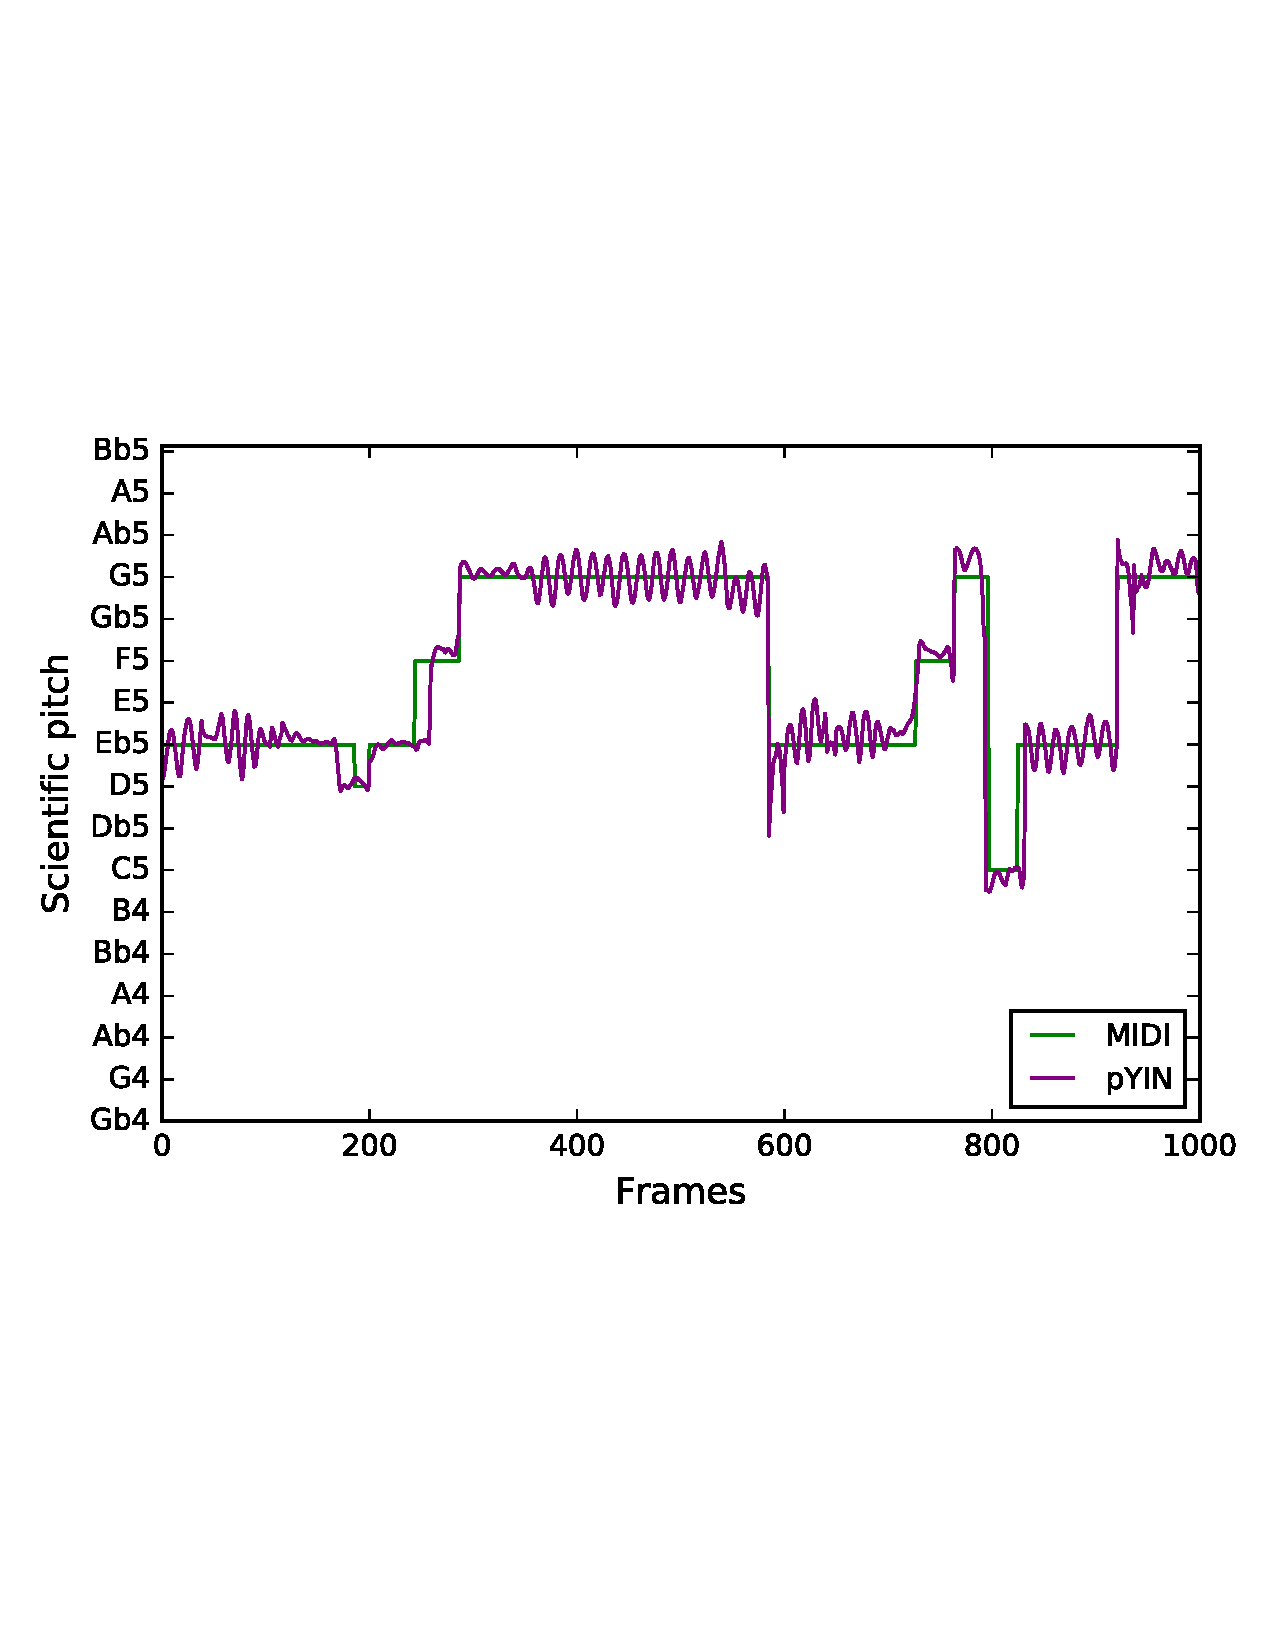
\includegraphics[width=0.5\textwidth]{figures/intonation_midi_and_pyin_aligned_active_54932280_1996063255.pdf}}\vspace{-1in}
    \subfigure{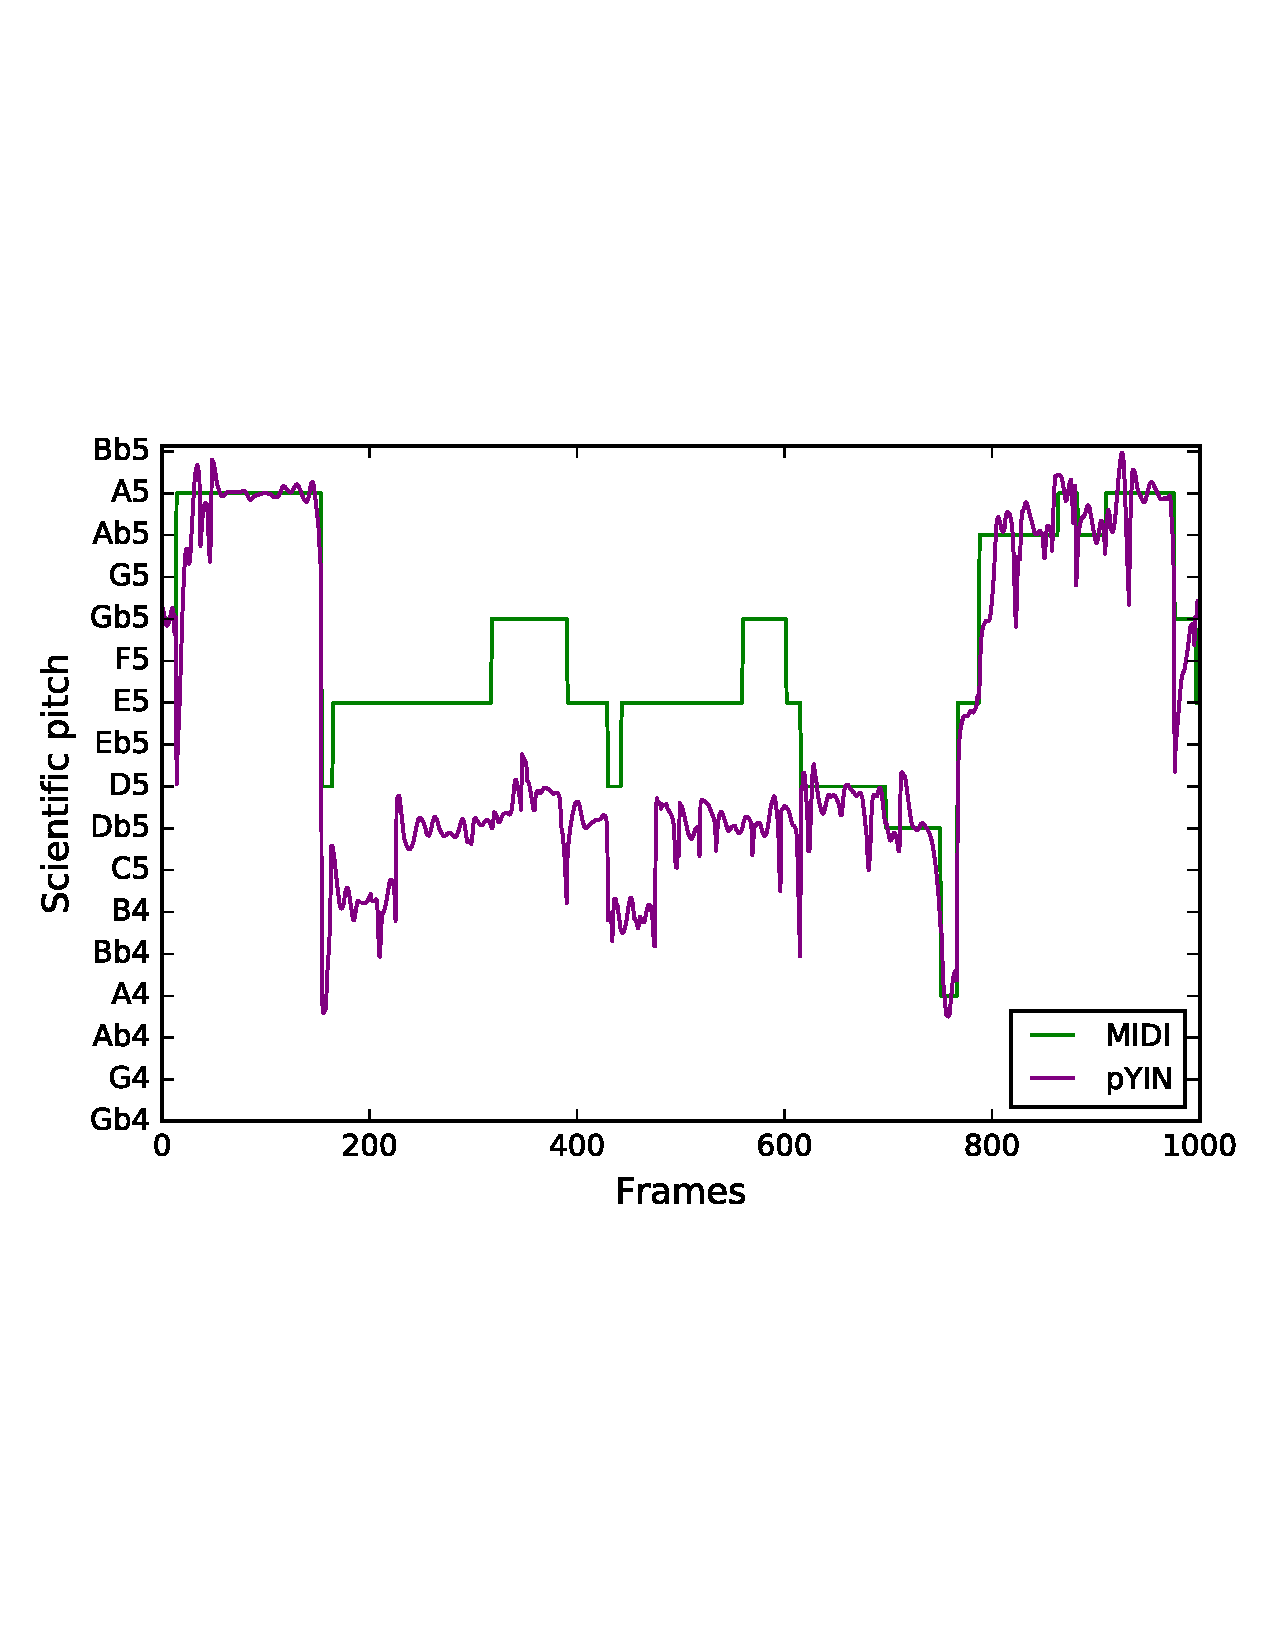
\includegraphics[width=0.5\textwidth, ]{figures/intonation_midi_and_pyin_aligned_active_544169967_2234781750.pdf}}\vspace{-1in}
    \subfigure{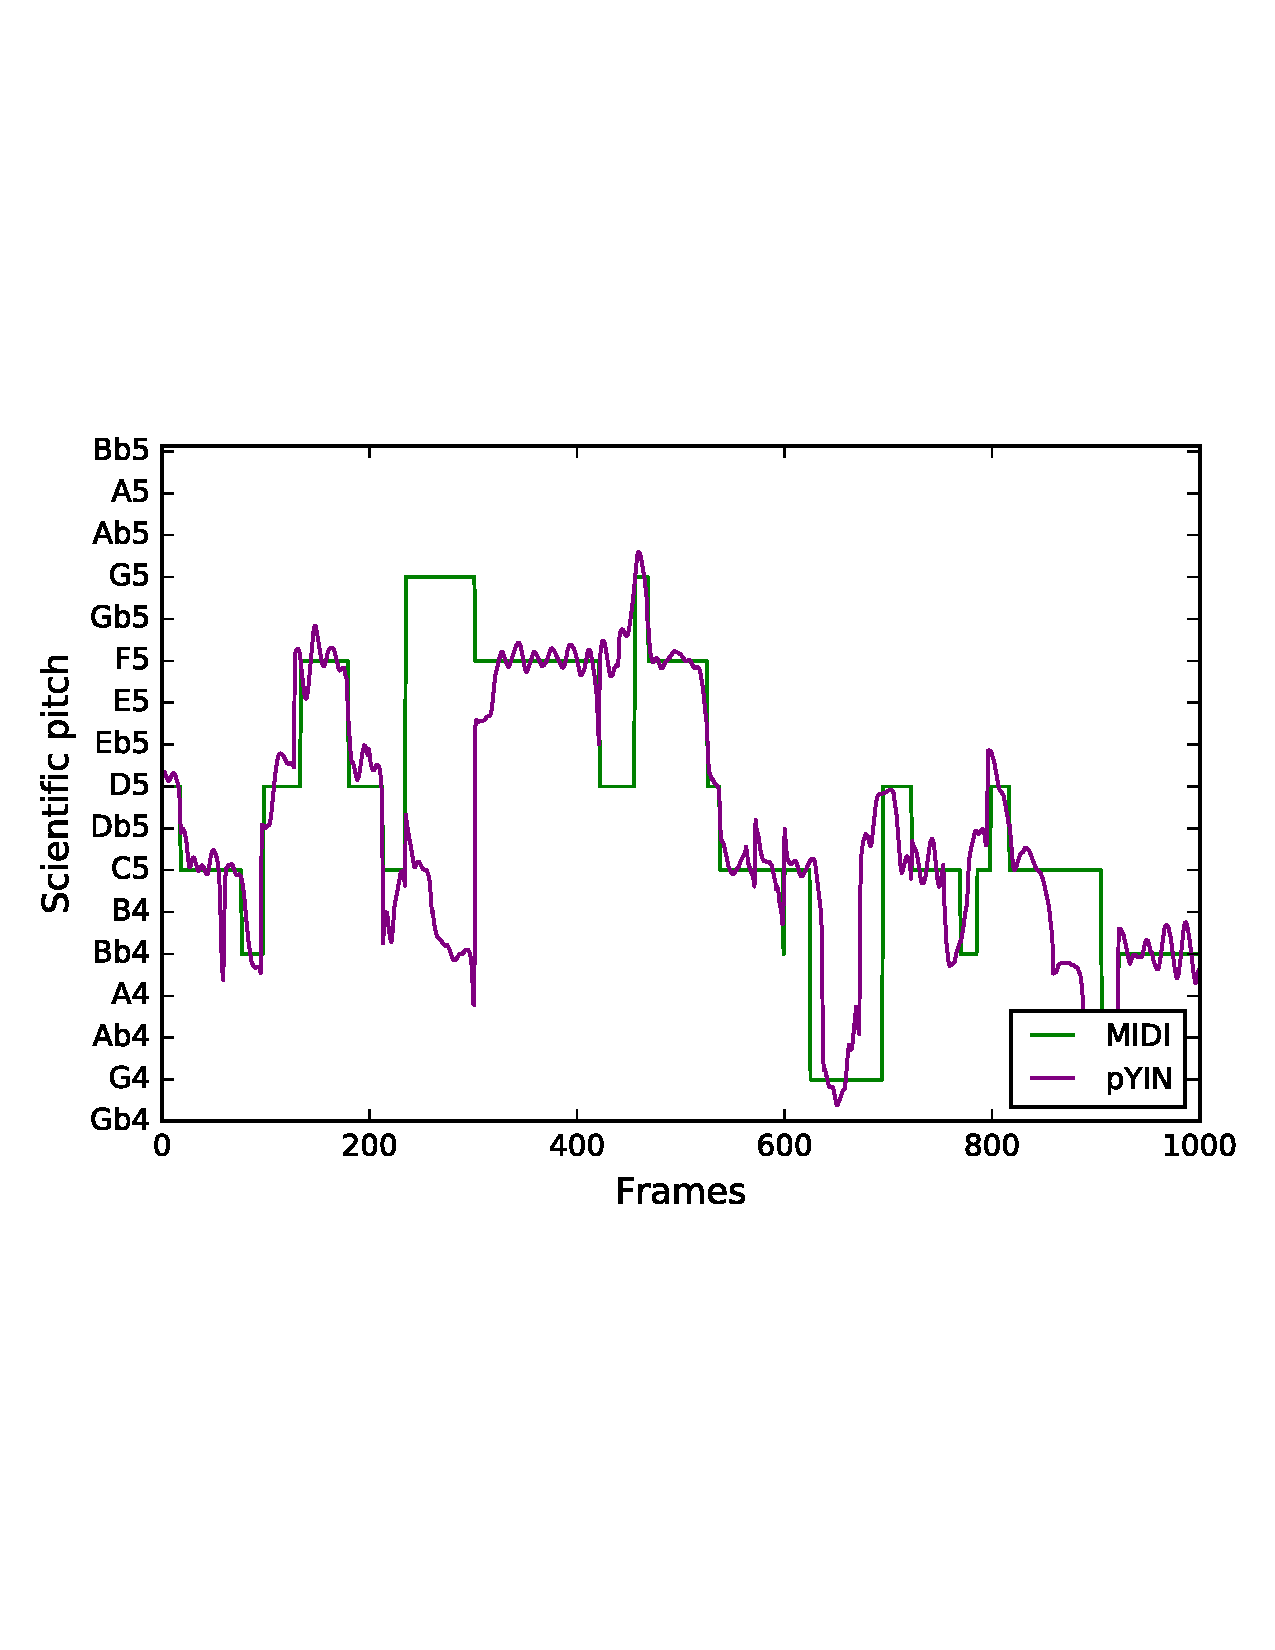
\includegraphics[width=0.5\textwidth, ]{figures/clustering_midi_and_pyin_aligned_active_545284262_2000375574.pdf}}\vspace{-0.5in}
    \subfigure{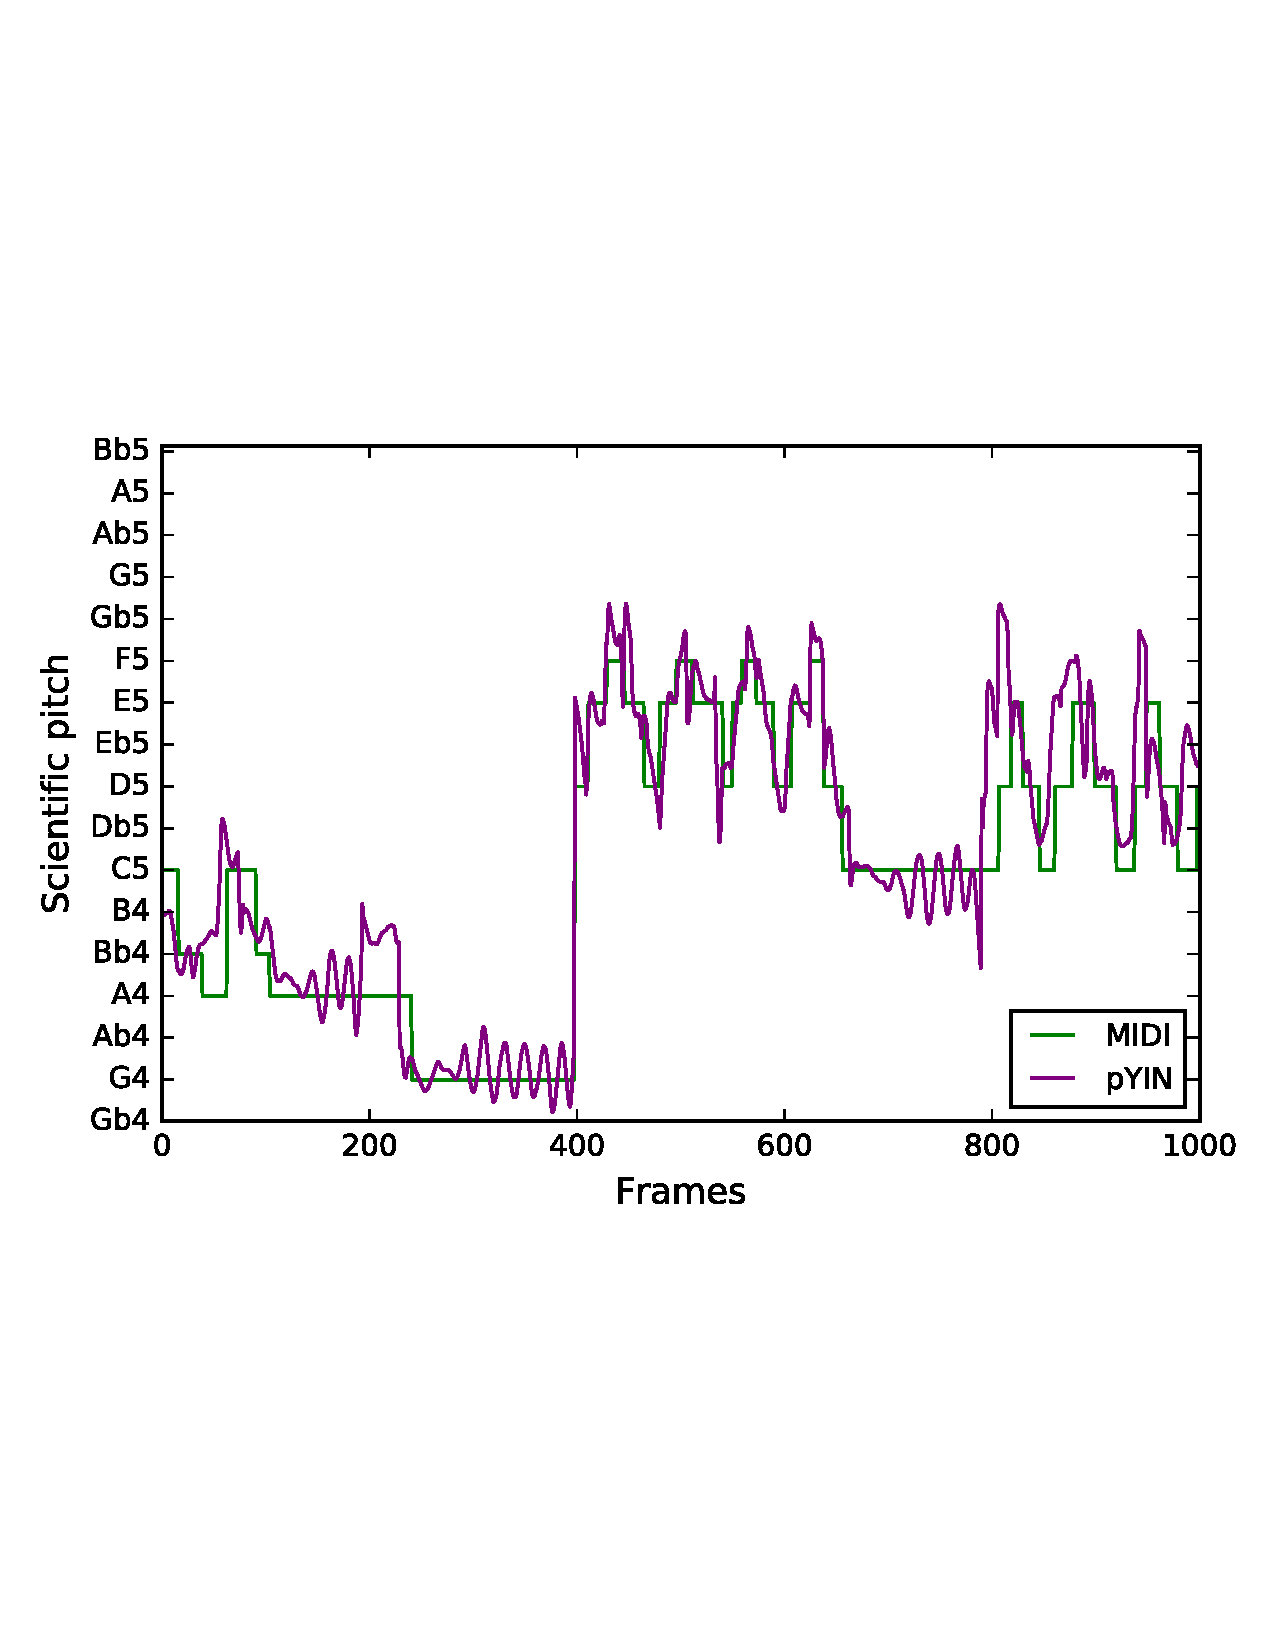
\includegraphics[width=0.5\textwidth, ]{figures/clustering_midi_and_pyin_aligned_active_54195986_1647186097.pdf}}\vspace{-0.5in}
    \caption{Singing pitch analysis of sample performances with aligned MIDI. Two are in the clusters selected for  ``Intonation'' dataset (top), two in the remaining clusters (bottom). Much can be learned about the individual performances. The top two appear more tightly aligned to the expected pitch, though the second plot contains harmonization at a major third below the musical score. The vibrato in the first plot is particularly smooth, a sign of an advanced singer. The third plot shows frequent deviation from the score, while the fourth shows deviation at the beginning and the end but accuracy in the middle, along with a smooth vibrato. Still, it is difficult visually determine from this data format whether a performance sounds ``in tune''.}
    \label{fig:sample_intonation}
\end{figure*}

%Related work
%- pitch deviation analysis
\section{Related work}
\label{sec:related}

\begin{figure}[h!]
    \centering
    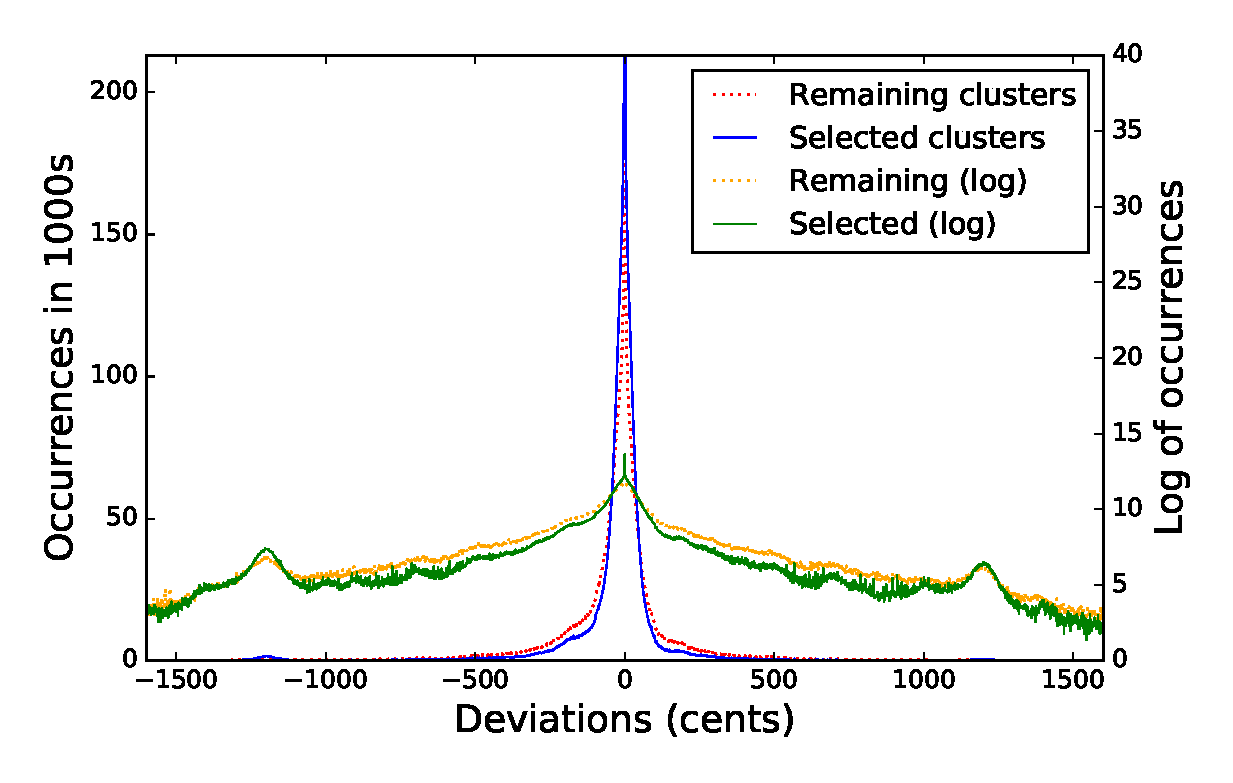
\includegraphics[width=\textwidth]{figures/full_histograms_comparison.eps}
    \caption{Global histograms of singing pitch deviations from the expected MIDI pitch in cents summed over 4702 performances in the ``Intonation'' dataset and 4702 in the remaining clusters. The plot is truncated at the top for readability. Scaled log histograms make more noticeable the small peaks at 1200 cents in both directions, due to octave deviations, common among singers. There is also, interestingly, a larger number of deviations between 100 and 300 cents in the negative direction than in the positive direction.}
    \label{fig:full_hist}
\end{figure}

\subsection{Automatic pitch deviation analysis}
Automatic analysis of musical intonation behavior has also been performed in other contexts. For example, Nichols \textit{et al.} \cite{nichols2012automatically} described an approach to discovering talented singers on YouTube based on features extracted mostly from the audio. One of the main features they chose consisted of a pitch deviation histogram, which characterizes intonation behavior of a full performance in a low dimension. Given that the performances were typically not associated with a musical score and that the singing was mixed with the accompaniment and other background sounds, the authors built the histogram from the Short-Time Fourier Transform amplitude peaks. A singer who sings flat should have a histogram skewed to the left, and an active vibrato will cause values to spread. Our feature extraction task is different from \cite{nichols2012automatically} because, as described below, we have access to the musical scores of the vocals and because the audio sources are separated. We can, therefore, apply a standard pitch detection algorithm to each vocal track and compare the results to the musical score. Comparison of performance pitch and musical score is also used by \cite{lim2010intune} in the context of a tool for musical performance visualization.


\begin{figure}[h!]
    \centering
    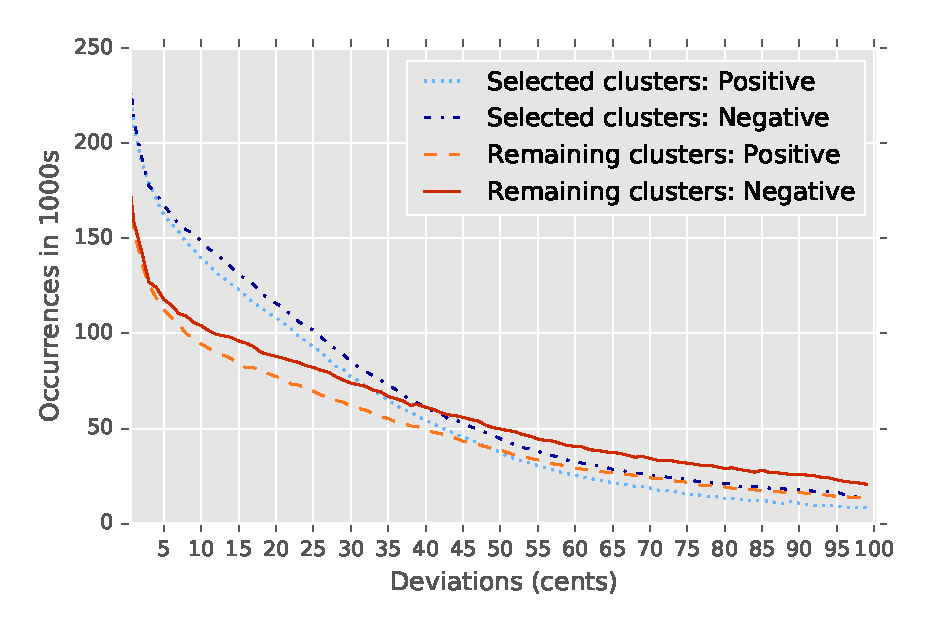
\includegraphics[width=\textwidth]{figures/full_pos_vs_neg_line.eps}
    \caption{Comparison of positive and negative deviation counts for cents ranging from 1 to 100 (omitting 0) for both datasets. In both groups, negative deviations are more common than positive ones. The ``Intonation'' dataset deviations are more concentrated around zero. }
    \label{fig:pos_neg}
\end{figure}

%Data collection and feature extraction
\section{Data collection and feature extraction}
\label{sec:features}
We collected solo vocal tracks of karaoke performances from a very large database. The first step was to filter for performances where singers used a headset---avoiding incorporating noise from the backing track into the recording. Given that we had access to a musical MIDI score of expected pitches, we also used a simple heuristic to filter for performances that were aligned enough with the score to exclude scenarios such as people speaking instead of singing. We kept this heuristic lenient enough that in-tune performances where the singer used harmonization (sang different pitches than the expected melody) or made other intentional deviations from the MIDI track wouldn't be excluded. This pre-filtering provided 14403 performances. 

The next step was to summarize intonation patterns of a performance using a low-dimensional set of features. The procedure is shown in Figure \ref{fig:pipeline} for two example performances. We first compared the singing pitch to the expected pitch in the MIDI score. We computed the singing pitch using the pYIN algorithm \cite{mauch2014pyin} on one minute of audio, starting at 30 seconds to avoid silence, with one sample (frame) per 11 milliseconds. pYIN has a high frequency resolution because it is based in the time domain and refines results using linear interpolation. Resolution is crucial for musical intonation, where a few cents difference can determine whether a pitch sounds in or out of tune. We shifted the MIDI score by a global constant to the octave nearest to the singing pitch, which can differ based on gender, age, and vocal type. We then computed the frame-wise absolute values of the difference in cents $\left| 1200 * log_2 \frac{f_1 + \epsilon} {f_2 + \epsilon} \right|$ between the performance and MIDI score. Of this set of values, we kept the differences less than or equal to 200 cents, equivalent to two semitones, in order to focus the analysis on intonation behavior when the singer was close to the expected pitch. Larger differences could be due to many reasons, ranging from misalignment of notes in time to harmonization, and might add undesired noise to the distributions. 

Finally, we summarized these variable-length sequences of frame-wise differences in a fixed, low-dimensional representation. We generated a random sample of 10,000 differences with replacement for every performance and kept 31 evenly spaced quantiles. This empirically chosen number is large enough to effectively summarize the characteristics of the distribution but produces a low enough dimensionality for clustering.

\begin{figure}[h!]
    \centering
    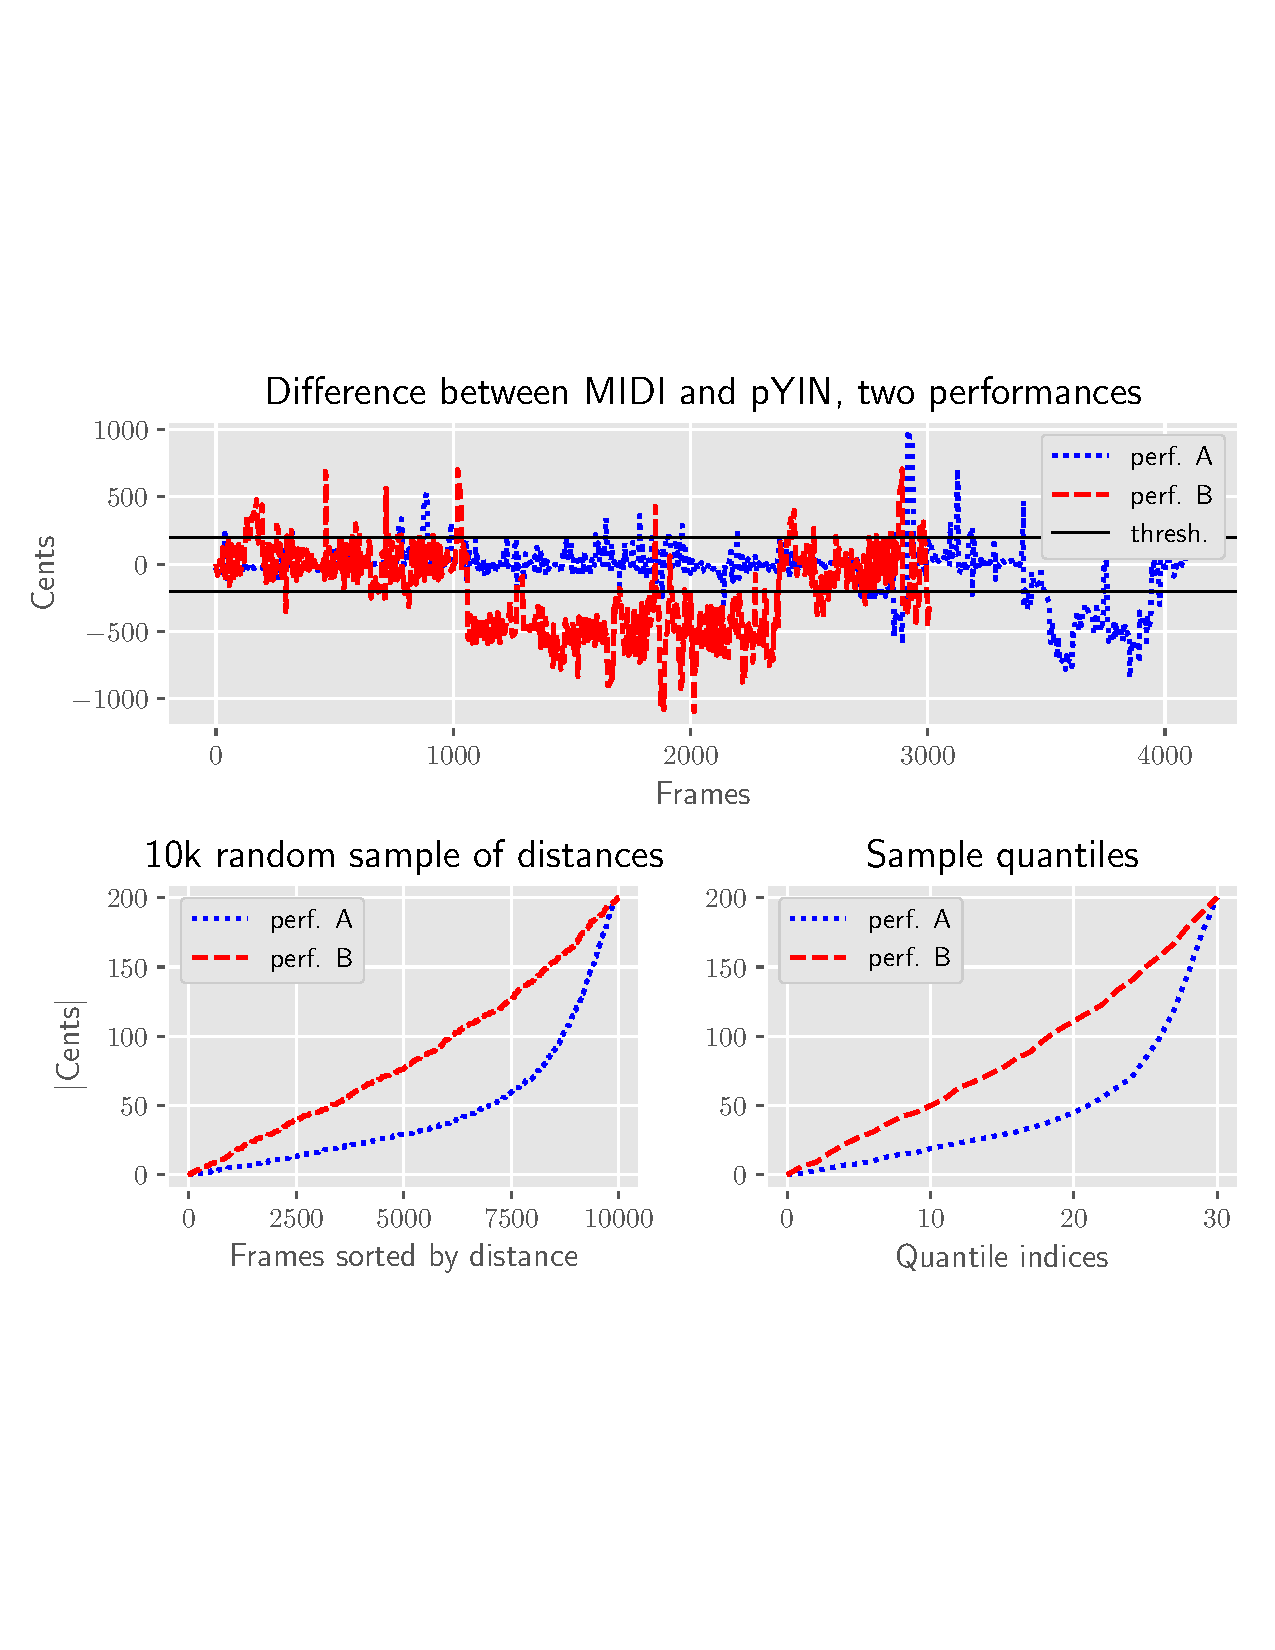
\includegraphics[width=\textwidth]{figures/data_processing_pipeline.pdf}\vspace{-1in}
    \caption{Data pre-processing steps for two example performances. The blue performance was selected for the ``Intonation'' dataset and the red performance was not. The first plot shows the frame-wise differences in cents between the measured singing pitch and equal-tempered MIDI score. We computed the absolute values of these differences and discarded those whose deviation was larger than 200 cents. The second plot shows random samples of 10,000 from the frame-wise difference lists, sorted by distance. The blue curve shows less deviation from the expected pitch than the red. The third plot shows 31 quantiles summarizing the curve in the second plot in a lower dimension.}
    \label{fig:pipeline}
\end{figure}
%Spectral clustering
% - genres and bias
\section{Spectral clustering}
As suggested by the studies described in Chapter \ref{chap:intonation}, an advanced singer might produce both smaller and wider pitch deviations, due to a pronounced vibrato or expressive variations such as pitch bending, time shifting, or harmonization, than a singer who sings close to the musical score but is slightly off pitch. For this reason, we didn't try to select performances based on a simple metric like average distance of singing pitch from the score. We also didn't attempt to directly model ``being in tune'', instead adopting a semi-supervised approach that clusters performances based on features generated from the deviations. We then chose which cluster to keep by listening to samples from each.

We applied spectral clustering to the summarized performances using the signless Laplacian matrix as the adjacency graph \cite{lucinska2012spectral}. This graph is based on selecting nearest neighbors (50 in our case). In practice, we clustered approximately 5000 songs at a time into 3 or 4 clusters, depending on which value produced better Newman modularity \cite{newman2006modularity}. We then listened to 50 samples from every cluster and subjectively determined the intonation of every performance by evaluating it as ``in tune'', ``neutral'', ``out of tune''. Consistently, one cluster produced distinctly good results with roughly 75 per cent of the songs classified as ``in tune'' and many of the remaining songs being classified as ``neutral'' rather than ``out of tune'', while the other clusters had only a small percentage of performances classified as ``in tune''. 

Keeping the samples from the selected clusters resulted in the ``Intonation'' dataset of 4703 performances. Though not every performance is in tune and not every performance in remaining clusters is out of tune, a majority of in-tune performances in this dataset suffices for many machine-learning applications.

\subsection{Genre, bias, and related challenges}
An undesirable outcome of this clustering approach was that musical genres were clustered along with intonation patterns. As described in Chapter \ref{chap:intonation}, different musical cultures and subcultures often have diverging traditions regarding musical intonation. In the Smule samples, a majority were of Western popular music, and the in-tune clusters tended to consist mostly of such music. I had planned to use performances from other clusters for testing, but realized that many of the performances were country, where singers deliberately might wish to sing flat, and the automatic pitch correction model trained on a different genre might not apply. As this was an intern project, I do not currently have the ability to update the clustering technique, and have to focus on the effects of the proposed system on Western pop music. In future work, if implementing this program for real-world use, I would first separate performances by genre, then apply spectral clustering within the genre. This improvement requires advanced genre classification, but this field is growing and improving quickly in the context of music recommendation systems.  

%Analysis
\section{Analysis}

The quality of the dataset is difficult to measure without a subjective listening test. At this point, we do not attempt to directly show that the ``Intonation'' dataset performances have better intonation than those in the remaining clusters. Instead, we show a difference in the intonation behavior distributions in the two collections. In order to compare samples of the same size, we analyzed the full ``Intonation'' dataset of size 4702 and a randomly selected a sample of the same size of performances from the remaining clusters.

\subsection{Data pre-processing for analysis}
We computed the frame-wise differences between singing pitch and MIDI score similarly to the way described in Section \ref{sec:features}. Unlike before, we retained the sign instead of taking the absolute value in order to know whether the pitch was sharp or flat. We also kept all deviations instead of discarding those larger than 200 cents: At the analysis stage, we are interested in intonation characteristics across the whole performance, including the larger deviations due to harmonization, expressive deviations, or inaccuracy. 

To minimize misalignment before computing the deviations, we applied Dynamic Time Warping (DTW) \cite{berndt1994using} to better align the MIDI and singing pitch tracks. This algorithm stretches both signals in time in a way that minimizes the total sum of distances between the two. We used the algorithm as described in \cite{muller2015fundamentals} and implemented in \cite{mcfee2015librosa}. To avoid distorting the pitch track, we forced the algorithm to apply most time warping to the MIDI, which consists of straight lines. We discarded frames where either the musical score or pitch tracks were silent in order to only consider active frames in our analysis. Figure \ref{fig:sample_intonation} shows four example performances after the initial processing. The top two are from the selected clusters and the bottom two from the remaining clusters.

\subsection{Pitch deviation histogram}
We compared the sequences of frame-wise pitch deviations from the selected clusters to those from the remaining clusters. Similarly to \cite{nichols2012automatically}, we computed histograms of the deviations from the equal-tempered MIDI score summed over all performances in each group, normalizing them to have the same total counts. Figure \ref{fig:full_hist} shows that the ``Intonation'' dataset deviations are more concentrated very close to 0 than those in the remaining clusters. The same can be observed at other harmonization peaks, $\pm1200$ cents (an octave) and other values in between, indicating more intentional harmonization and less accidental deviation. There is also, interestingly, a higher concentration of counts between 100 and 300 cents especially in the negative direction. This dataset is of amateur singing, so there is also a chance that some singers would be singing flat. However, this clearly visible peak might be due to intentional harmonization and expressive suspensions. 

\subsection{Pitch deviation probabilities}
We examined whether we could find intonation tendencies like those described in Section \ref{sec:empirical}. Unlike in the data used in the cited studies, the backing tracks are fixed recordings, so all pitch adjustments happen in the voice. This can affect the pitch deviation distributions. In Figure \ref{fig:pos_neg}, we examine deviations within 100 cents because a larger deviation corresponds a different note. Both collections tend towards negative deviations, but the tail is lighter in the selected clusters.

We quantify this result by estimating the probability of negative versus positive deviations within various absolute deviation thresholds using bootstrapping \cite{efron1994introduction} with 10000 iterations, as shown in Table \ref{table:1}. We choose ranges of cents that are of interest when comparing theoretical musical intervals generated using the equal temperament versus other intonation systems (e.g., Pythagorean or Just intonation, described in the cited studies). Use of other intonation systems would explain deviations of 2 to 16 cents. We first examine the ratio of deviations less than 2 cents. As expected, a probability of 0.5 shows no significant preference for sharp versus flat intonation. Within 2 to 16 cents, we get 0.51. However, the largest probabilities occur at larger values, 300 cents. We cannot determine whether this deviation is a desirable effect or due to an unknown factor. The tendencies are observed in both collections. 


\begin{table}[t!]
\centering
\begin{tabular}{ |c|c|c| } 
\hline
\multicolumn{3}{|c|}{Results from ``Intonation'' dataset (4702 performances)}\\
\hline\hline
Cents range & Negative/positive deviation ratio & Var \\
\hline
1 to 2 & 0.500 & 0.001 \\ 
2 to 16 & 0.506 & 0.001 \\ 
1 to 100 & 0.532 & 0.002\\ 
100 to 300 & 0.727 & 0.002\\ 
\hline\hline
\multicolumn{3}{|c|}{Results from other performances (9701 performances)}\\
\hline\hline
Cents range & Negative/positive deviation ratio & Var \\
\hline
1 to 2 & 0.500 & 0.001 \\ 
2 to 16 & 0.509 & 0.001 \\ 
1 to 100 & 0.541 & 0.002\\ 
100 to 300 & 0.700 & 0.002\\ 
\hline
\end{tabular}
\caption{Probability estimates of negative versus positive frame-wise deviations of singing pitch from the equal-tempered MIDI score, computed using bootstrapping. The analysis was performed within different ranges of interest. When the deviation is less than 100 cents, the singer did not sing a different note. We found a particularly strong tendency towards negative deviations in the range of 100 to 300 cents.}
\label{table:1}
\end{table}

%Dataset description and applications
\section{Dataset description and applications}
The ``Intonation'' dataset contains the full unmixed and unprocessed vocal tracks of 4702 performances. It consists of 474 unique arrangements by 3556 singers. It also contains the pYIN pitch analysis and multiple backing track features for the range of 30 to 90 seconds: constant-Q transform, chroma, mel-frequency cepstrum coefficients, root mean square error, and onset, all computed using the Librosa \cite{mcfee2015librosa} package. Metadata of the performances is included. The dataset has applications ranging from the study of singing style in the context of karaoke performances, with optional study of user meta-data, to machine learning. For example, the vocal tracks can be used for informed source separation, an approach similar to separation by humming, described in \cite{smaragdis2009separation} and \cite{liutkus2012informed}. Similarly, the dataset can be used for training a query-by-humming system, in a similar way to \cite{huq2010crowdsourcing}. The vocal pitch tracks and backing track features can be used to study automatic pitch correction applications trained on real-world singing and develop a proof-of-concept model for vocal pitch correction \cite{wager2018pitch}.

%Conclusion
\section{Summary}
We present a semi-automatic process for the task of searching through a large database of amateur karaoke performances for samples with a tendency for good musical intonation. The approach can be applied in other situations where a researcher needs to extract a subset of data samples from a large database. We show that the set of collected performances has a different intonation behavior distribution than the set of remaining performances. The resulting public dataset, ``Intonation'', of 4702 performances is available on the Stanford CCRMA DAMP website. The ``Intonation'' dataset can be used for music information retrieval applications like query-by-humming systems. Analyzing the dataset, we find that pitch deviations between the measured singing pitch and the MIDI score are more often negative than positive, implying that singers more often choose lower frequencies, use them unintentionally by singing flat, or decorate pitch contours with flat sections.